\section{Memory Transfer Optimization}
\label{sec:transfer}
\subsection{Pinned Memory}
\label{pinned}
One of the most important aspects of optimization is the memory transfer between host and device.\\
Unfortunely, as we have seen in \ref{tab:pci_comp}, the link bandwidth between host and device is by several times slower than access to device memory.\\
Memory transfer without modifications uses pageable memory to copy data from host to device and vice versa.\\
Using pageable memory is problematic, because as soon as the device requests access to host memory ( for example for memory copies)
the host has to check whether the data even resides in physical memory or if it has been swapped out.\\
This results in a non-trivial CPU load and therefore lowers the bandwidth.\\
To avoid this, it is possible to request so-called page-locked, or \emph{pinned memory} which is not eligible to swapping (? even access?).\\
Page-locked memory results generally in a much higher bandwidth, though this difference is influenced by the CPU where a system
with a stronger CPU performs better than a system with a weaker processor on pageable memory but in all instances slower than pinned memory.\\
Without the involvement of the processor, the OS has to fulfil the demand that page-locked memory is \textbf{always} backed by physical memory,
so the device can setup a direct memory access ( DMA).\\\\
Resulting into higher bandwidth and lower system load for the host, it is one of the simpliest yet most effective ways to improve memory transfer.\\
Using consumer-grade hardware the following data has been gathered to further display the differences in \ref{fig:bandwidth}.\\
\begin{figure*}[ht]
    \centering
    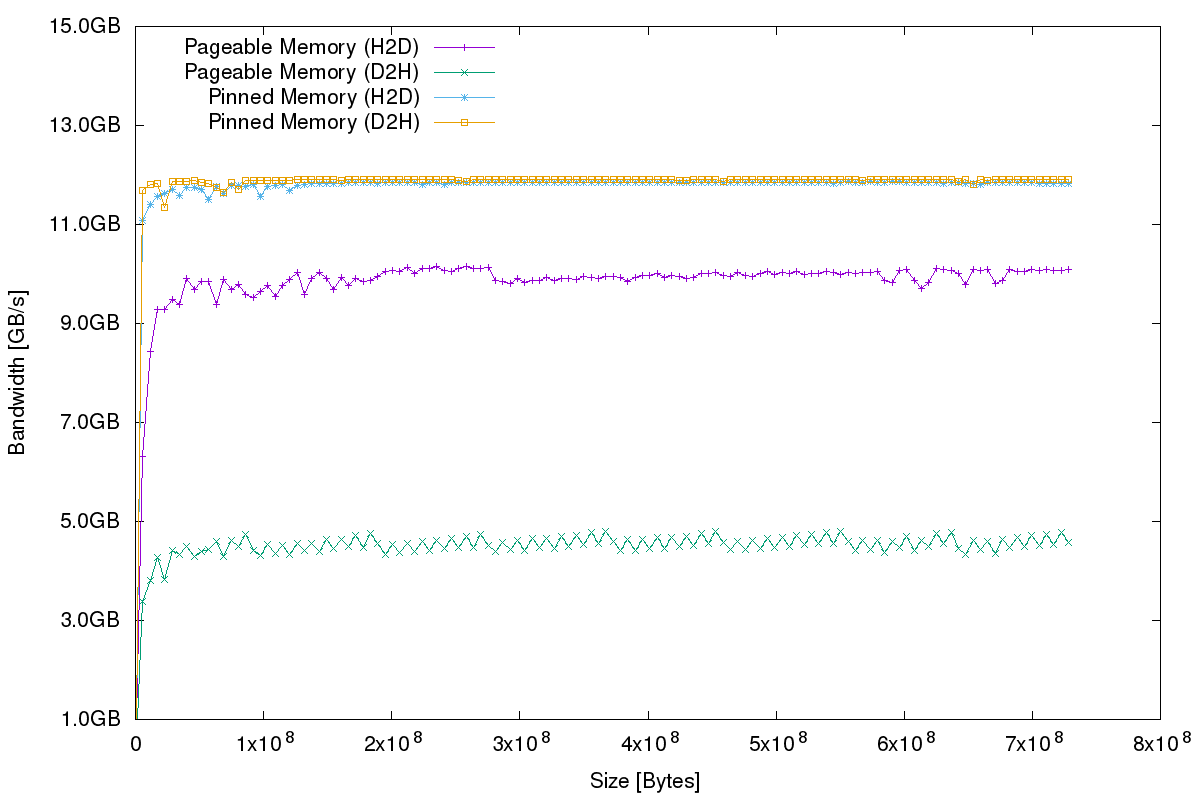
\includegraphics[scale=0.5]{media/bandwidth_pageable_vs_pinned_both.png}
    \caption{averaged bandwidth of 10 measurements on GTX 750 1GB, Intel(R) i5-4670 @ 3.40GHz}
    \caption*{Source code: \href{https://github.com/spotlight0xff/cuda\_paper/code/bandwidth}{On Github}}
    \label{fig:bandwidth}
\end{figure*}
% discuss results
These results have been recorded by allocating 128 different memory sizes (linearly distributed from 1 byte to roughly 700 MB) using respectively pageable and pinned memory.\\
To verify the data, these recordings have been averaged about 10 measurements.\\
The above figure shows clearly the significant speed-up provided by pinned memory, especially in the case of device to host transfer
whereas pinned memory shows no notable difference between the transfer direction.\\
Even though the overall results may be expected, the displayed disparity between the pageable memory transfers can be surprising. (explanation...?)\\\\

While host memory is page-locked, it can't be access and therefore used by the operating systems memory management,
which may result in degration of the systems performance due to insufficient memory available.\\
Another notable pitfall of pinned memory is the increased allocation time as we can see in the next paragraph.\\
\subsubsection{Registering Host Memory}
In some cases it is desirable to not allocate pinned memory, but to flag already allocated host memory as pinned memory.\\
This is especially interesting for applications with addon functionality where addons can provide host memory,
the application then registers it as page-locked using \emph{cudaHostRegister()}, operates on the accelerated memory and later unregister it with \emph{cudaHostUnregister()}.\\
\begin{table}
\centering
\begin{tabular}{c|c|c}
    \textbf{Size} & \textbf{Allocation} & \textbf{Registration}\\
\hline
\textbf{512 bytes} & 0.30 ms  & 0.08 ms\\
\textbf{1 MB}      & 0.28 ms  & 0.23 ms\\
\textbf{200 MB}    & 37.92 ms & 17.83 ms\\
\textbf{500 MB}    & 94.30 ms & 44.11 ms\\
\hline
\end{tabular}
\caption{Allocation times of pinned memory versus registering host memory}
\caption{System: GTX 750 1GB CC 5.0 with CUDA 7.5}
\caption{Source code: \href{https://github.com/spotlight0xff/cuda\_paper/code/alloc/}{on GitHub}}
\label{tab:host_reg_pinned}
\end{table}
As expected is marking host memory as pinned faster than allocation itself.\\
\subsubsection{Portable Pinned Memory}
Pinned Memory can be allocated or registered \emph{portable}  when it is required to access data on multiple CUDA units,
because an allocation made by one GPU is by default only accessible to the allocator.\\
As with the following two types of pinned memory, using it is as simple as setting a parameter in
\emph{cudaHostAlloc} or \emph{cudaHostRegister} to \emph{cudaHostAllocPortable} or \emph{cudaHostRegisterPortable} respectively.
Memory marked as portable is mapped and accessible by all GPUs on the system.\\
With UVA in effect, pinned memory is per default marked portable.
\subsubsection{Mapped Pinned Memory}
To map pinned memory directly into the GPU address space, enabling the developer to access 
in CUDA 2.2, it is possible to map pinned memory directly into the CUDA address space, which enables the developer to write directly to host memory.\\
This eliminates the need for device memory allocation, especially in a situation where data has to be only read or written once, it is preferable to use mapped memory instead of memory copies.\\
Using mapped pinned memory it is important to align the data properly to have its access coalesced as described in ~\ref{global_access}.
With UVA in effect, CPU and GPU share the same address space and therefore the same address can be used so there is no need to update both allocation tables.
\subsubsection{Write-Combined Pinned Memory}
TODO
\subsection{Zero-Copy}
\label{zerocopy}
Mapped Pinned Memory, or \emph{zero-copy},  is a feature introduced in CUDA 2.2 to allow direct access to host memory without explicit memory copies.\\
This is particulary useful if data is accessed sparsely or if the GPU is integrated.\\
On integrated GPUs zero-copy is always benefitial, because the host memory (most notable the RAM) and the GPU share the same physical memory. Therefore it is unnecessary to perform additional memory copies.\\
Another interesting use of mapped pinned memory is the ease with which it is possible to enable overlapping memory transfer with kernel execution.\\
Overlapping is normally performed using multiple streams where only parts of the memory is copied at once like illustrated in \ref{fig:overlapping}.\\
CUDA simplifies this process with zero-copy, where the data transfer is done transparently similar to the Unified Memory concept ( see \ref{unified_memory} ) where data is only transferred as needed.
This technique is only possible and benefitial due to DMA, because without it a host thread would've had to receive and perform the memory transfers accordingly, resulting in higher system load and lower bandwidth.\\
Additionally to overlapping, zero-copy can also be used to access complex structures without performing expensive deep copies, again similar to Unified Memory.\\
